\documentclass[11pt]{article}
\usepackage[margin=.75in]{geometry}
\usepackage{lmodern,amsmath,booktabs,graphicx,xcolor,pdflscape}
\usepackage[colorlinks=true,urlcolor=teal,citecolor=teal]{hyperref}
\title{Remaining-life error and the engines an inspection queue misses\\\large A split-engine simulation study with operating-condition stress}
\author{James Jean\\Independent research}
\date{28 October 2026\\GitHub research manuscript; not peer reviewed}
\begin{document}\maketitle
\begin{abstract}
A maintenance model is useful only if its error translates into a defensible inspection decision. This study fits fifteen prespecified configurations on NASA C-MAPSS simulated engine trajectories, separates fitting, tuning and uncertainty calibration by engine, and evaluates the frozen choice on two official test cohorts. In the matched-condition cohort, the selected histogram-boosting model reduces engine-balanced root mean squared error from 43.5 to 36.0 cycles and places ten near-failure engines in a ten-slot inspection batch, versus six for an age-only baseline. In the six-condition stress cohort, the corresponding error is 48.9 versus 47.7 cycles and the inspection count is eight versus nine in twenty-five slots. Calibration yields high observed trajectory coverage but broad intervals. The corrected numerical evaluation is retrospective because original test results had been inspected. The findings support examining error, transfer and constrained capture together. They do not establish performance on an operating fleet, maintenance savings or a safety guarantee.
\end{abstract}
\section{The decision behind the prediction}
An engine's estimated remaining life may support prioritization when inspection capacity is limited. Average prediction error does not directly measure which engines enter the queue. A model can improve predictions for long-lived engines while leaving the most urgent decisions little changed; a model that ranks the urgent engines well may still omit many when capacity is small. These are separate outcomes, so this study reports both.

C-MAPSS provides a reproducible simulation setting rather than evidence from commercial maintenance operations \cite{nasa,saxena}. The contribution here is a compact, auditable comparison of engine-balanced prediction error, finite-sample trajectory calibration and fixed-budget inspection capture. The regressors and calibration idea are established methods; neither algorithmic novelty nor an exhaustive literature gap is claimed. The experiment addresses the narrower question of whether a model selected for lower error retains its apparent operational advantage when the source operating-condition structure changes.
\section{Data and declared information boundary}
The NASA-linked archive contains simulated run-to-failure training trajectories, truncated test trajectories and remaining-life labels for the test endpoints. FD001 has one source-described operating condition and FD002 has six. Both use the same nominal high-pressure-compressor fault family. FD002 therefore supplies a dataset-level operating-condition stress comparison; the design does not establish that every individual test regime is unseen.

The FD001 training file contains 20,631 cycle rows for 100 engines. Engines 1--70 fit all models, 71--85 tune them and 86--100 calibrate uncertainty. These cohorts yield 18,731 eligible windows after requiring twenty observed cycles. The official test files contribute 100 FD001 engines and 259 FD002 engines, with 11,196 and 29,070 eligible windows, respectively. Source-local engine numbers are namespaced by file; equal numbers across files do not imply the same physical engine. No FD002 training data enter development.

The parser verifies twenty-six numeric columns, unique unit--cycle pairs and contiguous cycles beginning at one. It uses neutral labels for three operating settings and twenty-one sensors because the source's prose has an inconsistent final sensor-number example. No unsupported physical sensor names or units are assigned. Archive and member hashes, fixed public access URL and retrieval timestamp are retained. The source portal leaves licensing unspecified; raw members, the original paper and source README remain local. Only original code, derived evidence and retrieval instructions are published.

Training remaining life is the final cycle minus the current cycle. Test remaining life is the last observed cycle plus the supplied endpoint label minus the current cycle. Future failure information is used only for labels. Features are current age, current operating settings and sensors, and each sensor's trailing-twenty mean, population standard deviation and linear slope, including the current observation. No centered window, future sensor value or whole-engine normalization is allowed. This yields eighty-eight features. The original floating rolling-moment implementation selected different models on two Linux workers. Source-four-decimal integer sums, sums of squares and centered sums now construct sensor moments without cancellation in constant channels; checked bounds prevent integer overflow. Round-trip parsing and binary feature fingerprints make the input comparison explicit. The exact original-worker cause was not isolated because those feature fingerprints were not retained. This correction leaves the model grid, split, target and numerical tolerance unchanged, preserves original results, and does not create a new confirmatory test.
\section{Optimization, calibration and test plan}
The age-only baseline subtracts current cycle from the mean failure age of the seventy fitting engines and clips negative predictions at zero. The search also includes six 160-tree random forests, crossing maximum depth 4, 8 or unlimited with minimum leaf size 5 or 20, and eight histogram-boosting configurations, crossing depth 2 or 3, learning rate 0.05 or 0.1, and L2 regularization 0 or 1. Boosting uses one hundred iterations, minimum leaf size twenty and no early stopping. Seed 20261028 and two computation threads are declared; no pretrained model is fine-tuned.

Each engine receives equal total fitting weight. Selection minimizes the tuning mean of engine-specific MSE, with candidate-name tie breaking:
\[
 L=\frac{1}{E}\sum_{e=1}^{E}\frac{1}{n_e}\sum_{t=1}^{n_e}(\widehat y_{et}-y_{et})^2.
\]
All fifteen results, runtimes and predictions are retained. The winner is depth-two histogram boosting, learning rate 0.1 and L2 regularization zero. The learning rate is at the boundary of the finite search; a global optimum is not established. The original configuration and calibration radius were committed before the first test command. A later numerical correction followed inspection of that test, so the corrected results below are retrospective.

For each of the fifteen calibration engines, the nonconformity score is its maximum absolute residual over eligible observed windows. The nominal 90\% trajectory radius is order statistic $\lceil(15+1)0.9\rceil=15$, the largest score. Intervals are $[\max(0,\widehat y-q),\widehat y+q]$. The selected and baseline radii are 161.8 and 139.1 cycles. This trajectory construction assumes exchangeability across engines; observed coverage cannot prove that assumption, especially under condition shift.

Each test engine contributes its last available window to one benchmark batch. Inspection capacity is $\lfloor0.1E\rfloor$. Engines are ranked by the lowest predicted remaining life, rounded to eight decimal places, then by local ID. The main horizon is true remaining life at most thirty cycles; fifteen and sixty cycles are prespecified secondary horizons. The batch is not a synchronized real fleet, and outcomes outside a horizon are not automatically economic false positives.
\section{Results and their practical limits}
\begin{table}[ht]\centering\small
\caption{Frozen evaluation. RMSE is engine-balanced and inspection results use the thirty-cycle horizon.}
\begin{tabular}{llrrr}\toprule
Test & Model & RMSE, cycles & Captured/inspected & Horizon recall\\\midrule
FD001 & Age-only & 43.5 & 6/10 & 24.0\%\\
FD001 & Selected sensor & 36.0 & 10/10 & 40.0\%\\
FD002 & Age-only & 47.7 & 9/25 & 14.8\%\\
FD002 & Selected sensor & 48.9 & 8/25 & 13.1\%\\\bottomrule
\end{tabular}\end{table}

The selected model reduces FD001 engine MSE by 599 cycles squared. A two-thousand-draw paired-engine bootstrap gives a conditional 95\% percentile interval of $[-901,-323]$. In FD002 the difference is $+117$, with interval $[-174,396]$. Resampling uses engines rather than overlapping windows. These intervals describe the benchmark cohorts and fixed analysis; they are not population or production guarantees.

The matched-condition batch contains twenty-five engines within thirty cycles of failure. Capturing ten improves on the baseline but still omits fifteen because the queue has ten slots. In FD002 there are sixty-one near-horizon engines, and the selected model captures eight. Its inspection precision is 32\%, versus 36\% for the baseline. At the sixty-cycle horizon the baseline captures seventeen and the selected model 15. The chosen model therefore does not dominate every decision horizon. The age-only model also produces clipped-zero ties, making the declared ID tie rule consequential and visible rather than hiding it in an unstable sort.

The selected model covers every eligible window of all 100 FD001 engines and 257 of 259 FD002 engines. Mean interval widths are approximately 278 and 301 cycles. High coverage with such broad intervals does not make an inspection date precise. The baseline intervals are narrower but still broad, about 245 and 241 cycles, and completely cover 100 and 255 engines. The error advantage, inspection capture and uncertainty width must be assessed jointly.
\section{Verification and next experiment}
Independent scalar calculations reconstruct every exported MSE/MAE, source-derived target, calibration maximum and order statistic, interval, coverage, inspection ranking and bootstrap interval. Six contracts check future-value isolation, engine boundaries, label exclusion, equal engine weight and budget/tie handling. An independent source-window audit checks all twenty-one sensor summaries for six declared windows per partition; this is a spot audit rather than a second exhaustive feature implementation. A temporary-directory replay refits all configurations and checks required outputs at absolute tolerance $10^{-7}$ and relative tolerance $10^{-9}$.

The source is simulated, the cohorts use one fixed split, and the search is small. Uncertainty calibration is based on only fifteen engines. The study includes no real inspection calendar, failure consequence, parts cost or intervention-effect evidence. Its appropriate next experiment is operating-condition-aware development evaluated on genuinely new protected engines, followed by a separate costed scheduling study on permitted operational data. Reusing the current test after tuning would require a retrospective label. No safety, savings, deployment or commercial adoption claim follows from these results.
\begin{thebibliography}{9}\small
\bibitem{nasa} NASA. C-MAPSS Jet Engine Simulated Data; PCoE Data Set Repository. \href{https://data.nasa.gov/dataset/cmapss-jet-engine-simulated-data}{Dataset description} and \href{https://www.nasa.gov/intelligent-systems-division/discovery-and-systems-health/pcoe/pcoe-data-set-repository/}{official source repository}. Accessed 28 October 2026.
\bibitem{saxena} A. Saxena, K. Goebel, D. Simon and N. Eklund. Damage Propagation Modeling for Aircraft Engine Run-to-Failure Simulation. PHM 2008. Dataset attribution: A. Saxena and K. Goebel, NASA Ames, 2008.
\end{thebibliography}
\clearpage\begin{landscape}
\thispagestyle{plain}\centering
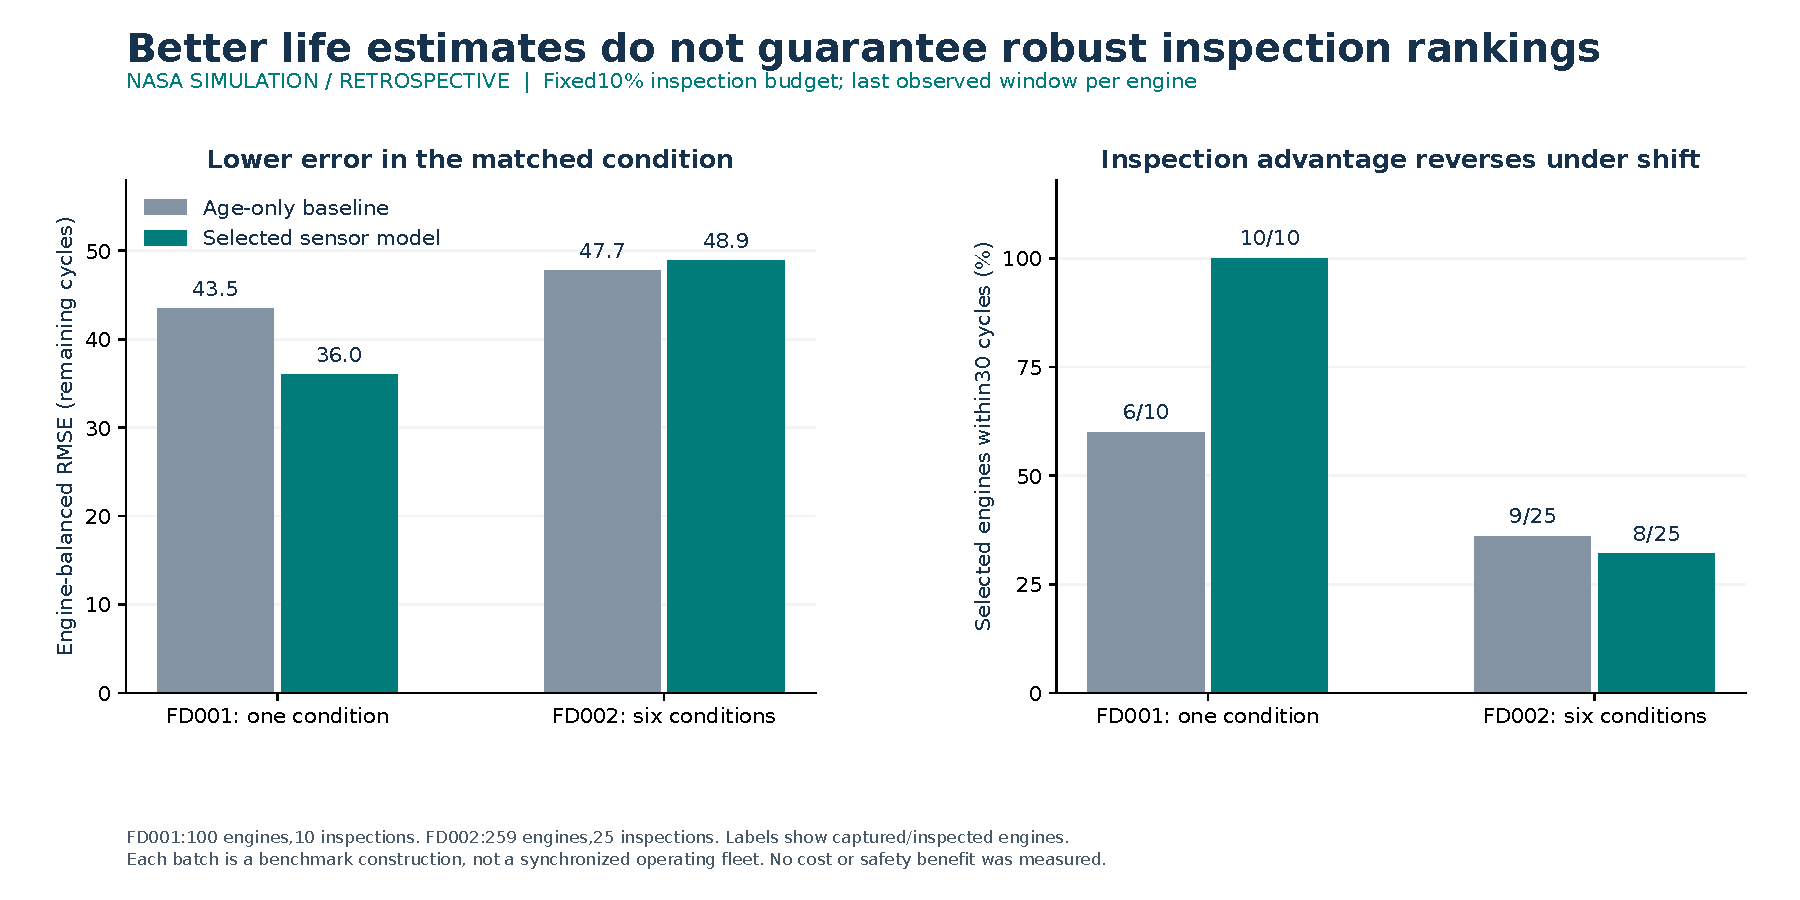
\includegraphics[width=.98\linewidth,height=.86\textheight,keepaspectratio]{images/decision-summary.pdf}
\par\small Figure1. Fixed-budget capture and error answer different questions. All trajectories are simulation data. Numerical labels count captured/inspected engines.
\clearpage
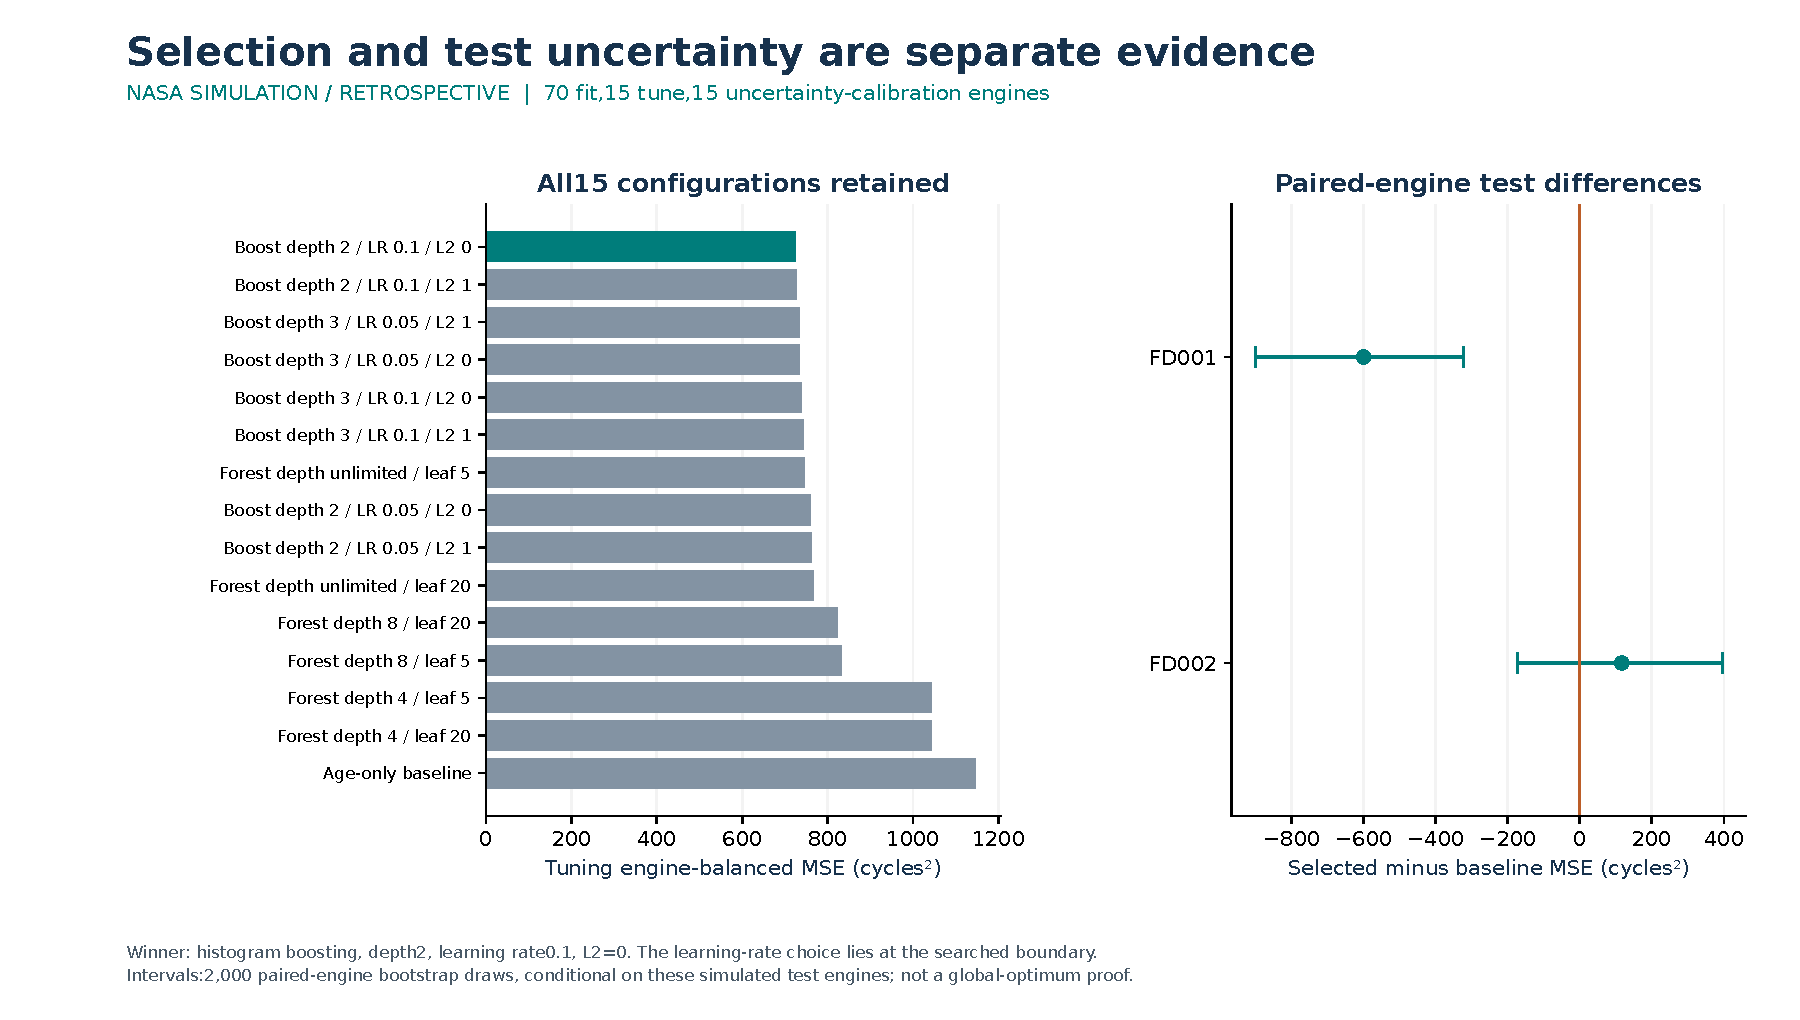
\includegraphics[width=.98\linewidth,height=.86\textheight,keepaspectratio]{images/optimization-evidence.pdf}
\par\small Figure2. The full finite search and paired-engine test uncertainty. A test interval crossing zero in FD002 limits the transfer claim.
\clearpage
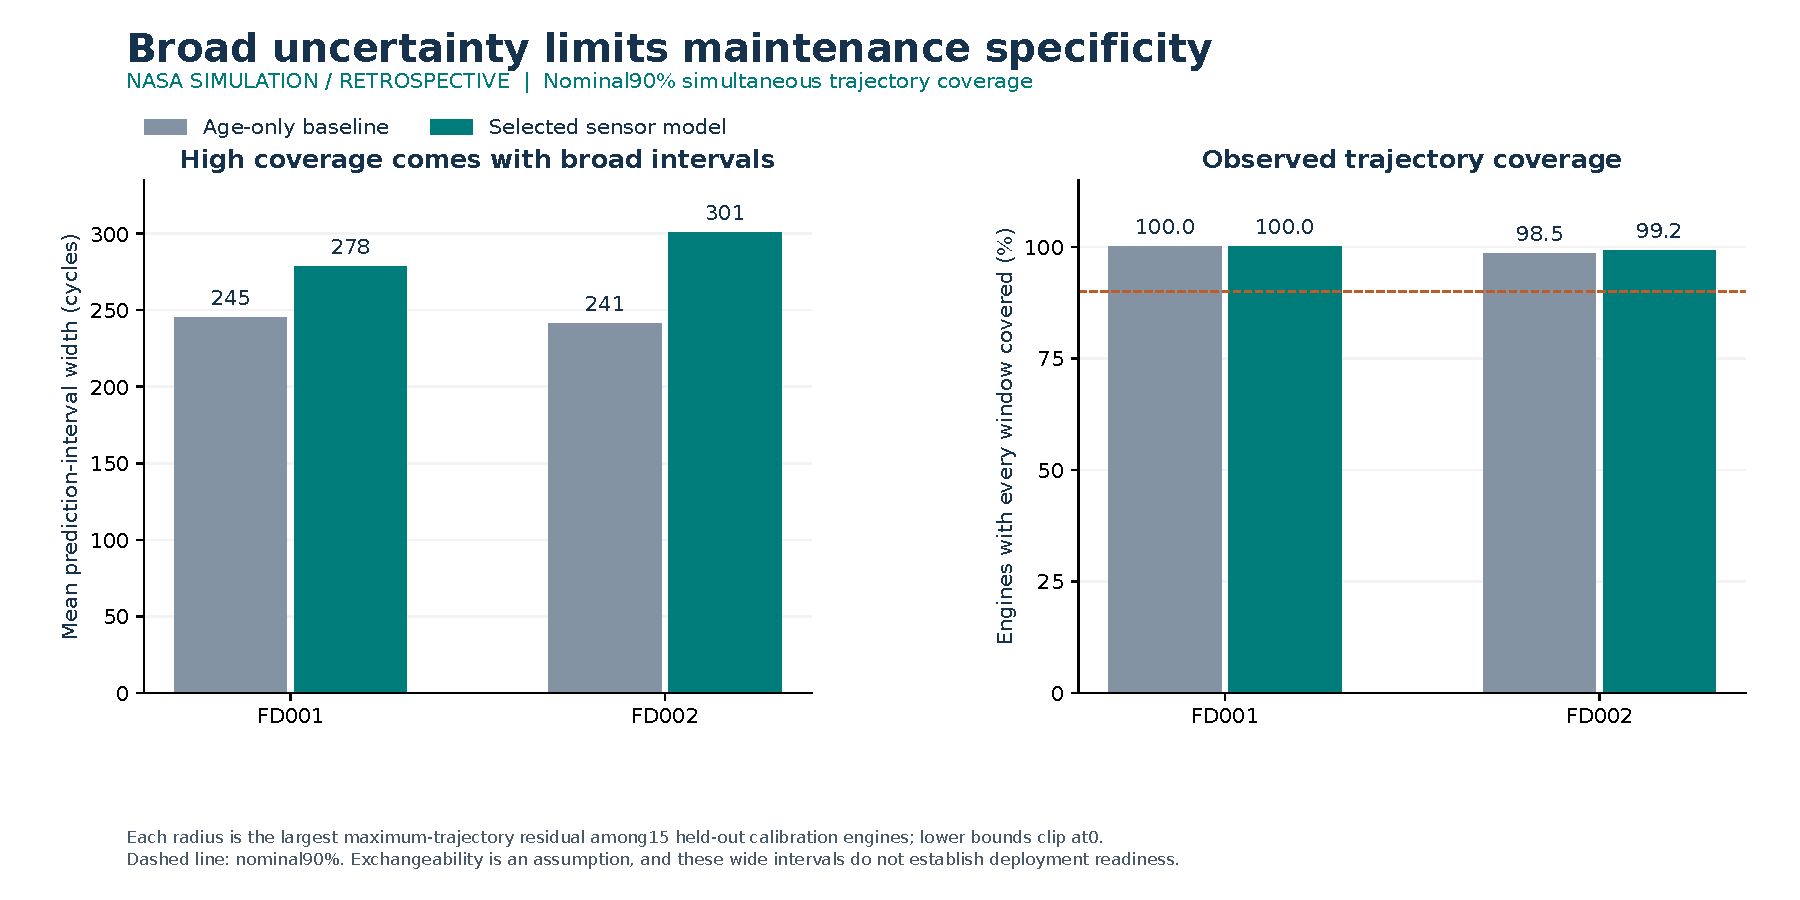
\includegraphics[width=.98\linewidth,height=.86\textheight,keepaspectratio]{images/uncertainty-tradeoff.pdf}
\par\small Figure3. Broad intervals deliver high observed trajectory coverage but limited maintenance specificity. The dashed line is the nominal calibration target.
\end{landscape}
\end{document}
